% Benchmarking in Unity
% https://blogs.unity3d.com/2018/09/25/performance-benchmarking-in-unity-how-to-get-started/
% Maybe try VRWorks https://developer.nvidia.com/vrworks

% Questions to answer in the evaluation chapter:
% \begin{enumerate}
%   \item{How big can the graph be so that it is comfortable visualizing the network?}\\
%   What is comfortable? Number of FPS?
%   How can we scale the graph? By adding nodes and spread them around, by adding more interconnexions?
%   Should the experiment split in several parts? Scaling, filtering, moving around, etc.
%   What is the performance by using Oculus Link and the performance using just the Quest hardware?
%   -We can use the Unity GPU Profiler for Oculus Quest and Go in order to see the performance.\\
%   \href{https://developer.oculus.com/blog/getting-started-w-the-unity-gpu-profiler-for-oculus-quest-and-go/}{See: Getting Started w/ The Unity GPU Profiler for Oculus Quest and Go}
%   \item{How is this way of visualizing the graph better by using VR?}\\
%   We are researchging the technology and the test with actual users is for future work.
%   \item{In what way can the application and the visualization of the graph be improved?}\\
%   Argue in the discussion part.
% \end{enumerate}

% Links
% Profiler panel

As part of the evaluation of our prototype, we wrote a list of questions focusing on performance and quality and that we will try to answer along this chapter. These questions are:
\begin{enumerate}
  \item For which interactions do we achieve the recommended FPS (72) for large biological networks?
  \item What network properties influence the scalability?
  \item Do we achieve the recommended FPS (72) for large biological networks when using the standalone Oculus Quest?
  % \item Bonus: how will “beautifications” influence scalability?
  \item How do users perceive the visualization of large biological networks in GeneNet VR?
\end{enumerate}

\section{Methodology of experiment setup}
% An experimentation plan was designed to ensure that the experiments are consistent and that they can be reproduced several times in order to get realistic measurements. We take into consideration the following aspects for our experiments:
% \begin{enumerate}
%   \item Scalability for different interactions.
%   \item Network characteristics.
%   \item Bottlenecks.
%   \item User study.
%   \item Hardware and software specification.
% \end{enumerate}

GeneNet VR has been developed to explore large biological networks that contain genetic information. We have used two datasets from the MIxT project \cite{dumeaux_fjukstad_interactions_tumor_blood} and built a use case where we try to solve visualization and scalability problems.

The performance is an aspect of GeneNet VR that we want to evaluate. Without a good performance, visualization tools like this one can become tedious to use. Also, smooth interactions are needed, so that the user can easily explore the networks to find information and patterns in them. We will evaluate the performance sor the interactions that are commonly used when exploring networks in GeneNet VR and that involve manipulating the position or size of the network or showing the edges. These are translate, scale and select nodes in the network. Because of time limitation, we couldn't evaluate other interactions. We will also evaluate if the number of nodes and edges influence in the scalability of the application. We will also study if there are bottlenecks and what is causing them. In Table \ref{tab:network-elements}, we show the elements that compose the networks that we used and how they can influence in the scalability.

\begin{table}[h!]
\centering
\begin{tabular}{l p{9cm}}
\hline
Element & Description \\
\hline
Clusters & The algorithm used to create the clusters is run during the initialization of the system, before the user can start exploring the networks. This can be time consuming because it involves many operations to process the text files (they have several thousands of lines). However, this is only processed once. \\
Nodes & Represented as 2D squares in the space, they consist of 2 triangles. They are always showing in the scene and their position change while scaling, translating and morphing the network.  \\
Lines & They represent relationships between the nodes. Every time a node is selected, line objects are created in the scene. They are 2-dimensional and consist of 2 points. Depending on the node we might need to render several hundreds of these lines in the scene. \\
\end{tabular}
\caption{Elements of the network that have influence in the scalability.}
\label{tab:network-elements}
\end{table}

In the website of Oculus, we can find a reference with the Oculus' performance baselines that an application should meet \cite{oculus_performance_baselines} and that we will follow during the evaluation. These are the following:
\begin{itemize}
  \item 72 FPS for Oculus Quest (required by Oculus).
  \item 50-100 draw calls per frame.
  \item 50,000-100,000 triangles or vertices per frame.
\end{itemize}

We will also evaluate the performance of the application being run on the Oculus Quest hardware, and compare it with the performance in the PC. The hardware of the Oculus Quest is not as powerful as the one of the machine that was used for the development. We would like to know if the performance on the Oculus headset is good enough for the visualization of datasets like the ones from MIxT.

As for the hardware specification, we ran the experiments in a machine with Windows 10. In Table \ref{tab:machine-specs}, we can see the hardware specification for the machine. The GPU of the machine is also specified in Table \ref{tab:gpu-specs}. The hardware specification of the Oculus Quest is shown in Table \ref{tab:oculus-specs}.

\begin{table}[h!]
\centering
\begin{tabular}{ll}
\hline
Processor   & Intel(R) Xeon(R) CPU E3-1275 v6 @ 2.80GHz 3.79 GHz \\
\hline
RAM & 64.0 GB                                            \\
System type & 64-bit Operating System
\end{tabular}
\caption{Machine specification.}
\label{tab:machine-specs}
\end{table}

\begin{table}[h!]
\centering
\begin{tabular}{ll}
\hline
Adapter type   & NVIDIA GeForce GTX 1080 Ti \\
\hline
Chip Type  &  GeForce GTX 1080 Ti \\
Available memory & 45025 MB
\end{tabular}
\caption{GPU specification.}
\label{tab:gpu-specs}
\end{table}

\begin{table}[h!]
\centering
\begin{tabular}{ll}
\hline
Panel Type   & Dual OLED 1600x1440 \\
\hline
Supported Refresh Rate  &  72Hz \\
Tracking & Inside out, 6DOF \\
CPU & Qualcomm® Snapdragon 835 \\
GPU & Qualcomm® Adreno™ 540 GPU \\
Memory & 4GB total
\end{tabular}
\caption{Oculus Quest specifications.}
\label{tab:oculus-specs}
\end{table}

We built a benchmark in Unity in order to run the experiments several times. We used the same version of Unity as in the prototype, version 2018.4.10f1. The 3D rendering API that we have used is OpenGL. In total, we ran each experiment 4 times and we showed an average of the results using tables and graphs. The experiments are coded in the benchmark using scripts so that we can reproduce them several times. For the networks translation and network scale interactions, we use mathematical functions to translate the network around the scene and to scale the network up and down. For the node selection we have chosen a set of nodes.

We measured the frame time (time the a frame takes to render), to analyse the performance. In Unity, the frame time is stored in a variable named deltaTime from the Time class. In order to find bottlenecks, we used a profiling tool from Unity. A profiler is used to get an overview of the performance of the application. This gave us information about per-frame CPU performance metrics. In addition, Unity also provides some metric information that we can be displayed in the Unity editor. We got information about the number of vertices in the scene and the number of triangles.

% Finally, we want to know how the users perceive the interaction and visualization of the network. We will evaluate this with a qualitative method with a demo of the application using the MIxT datasets and also an interview.

To evaluate the quality of GeneNet VR, we conducted a series of interviews with several employees from UiT involved in computer science and biology research projects. These interviews were conducted in an informal way and have the purpose of obtaining feedback about aspects like the research contribution in bioinformatics, the performance of the application and the interactions, the usability and also improvements that can be done to the project.

\section{For which interactions do we achieve the recommended FPS (72) for large biological networks?}


The experiments from this section were run on the PC and we used the blood dataset from MIxT. We chose this dataset because it is the largest one. We also ran each experiment for different sizes of the dataset: the whole dataset (2693 nodes), half size of the dataset (1346 nodes) and a third part (897 nodes). We didn't run the experiments using larger datasets and also on the Oculus Quest due to lack of time.

Each experiment lasts for 700 frames, starting from frame number 501 until frame 1200 in the application's timeline. We start from frame number 501 because some slowliness occurs during the  first frames, due to the initizalization of the application. In order to evaluate the experiments, we stored the frame time for each frame for a total of 700 frames. The frame time is the time that a frame takes to render. We use this value to determine if the application meets the 72 FPS. Once we obtain all the frame times, we extract the following averages for each experiment: the average frame time of all the frames, the average of the 0.25\% worst times and the average of the 1\% worst times.

The average of all the frames is the most important value to look at, because it can give us an idea wether the experiment meets the required FPS or not. In a perfect application where all the frames last the same amount of time and where the frame rate is 72, each frame would last around 13.9 milliseconds. However, this is not the case in real applications. If the general average is above the 13.9 milliseconds, it means that the experiment didn't pass the 72 FPS. By looking at the 0.25\% worst frame time and the 1\% worst frame time, we will get the frame with the worst time and the 7 frames with the worst times respectively (our experiments last for 700 frames). If we see that these frames have much worse times, compared with the general average, we will use a profiler to see if there are bottlenecks and try to give a solution to them.

% Draw calls: https://medium.com/@toncijukic/draw-calls-in-a-nutshell-597330a85381
% Basically a draw call contains all the information telling GPU about textures, states, shaders, rendering objects, buffers, etc. encapsulated as CPU work that prepares drawing resources for the graphics card. Converting state vectors (all the information mentioned before) to hardware commands for the GPU is very “expensive” for the CPU and API complexity becomes API overhead that does not help.

\subsection{Translating the network meets the 72 FPS}
In thise experiment, we evaluate the performance when translating the network. In the benchmark, the network is moved around in the scene using a sine function in the y axis and a constant function in the z axis. For every frame we update the y and z position of the network object. In Table \ref{tab:experiment_moving}, we can see the results that we obtained.

\begin{table}[h!]
\centering
\begin{tabular}{llll}
\hline
Dataset size & 0.25\% average low & 1\% average low & Average \\
\hline
size & 20.11 & 12.17 & 6.55 \\
size/2 & 22  & 12.79 & 6.5 \\
size/3 & 23.28 & 13.52 & 6.5 \\
\end{tabular}
\caption{Performance results in milliseconds when translating the network.}
\label{tab:experiment_moving}
\end{table}

The averages for all the sizes are below 13.9 milliseconds, so translating the blood dataset network meets the 72 FPS. There isn't a significant difference between the averages for the different network sizes. This is because the network that we are using is probably too small. It would be interesting to use larger networks to find out for which network size the performance is no longer good enough.

% Standard deviation? In statistics, the standard deviation is a measure of the amount of variation or dispersion of a set of values. A low standard deviation indicates that the values tend to be close to the mean of the set, while a high standard deviation indicates that the values are spread out over a wider range.

\subsection{Scaling the network meets the 72 FPS}
We also evaluated the performance when scaling network. We used a sine function as well and update the size of the network object for every frame to scale it up an down. In Table \ref{tab:experiment_scale} we can see the results that we obtained.

\begin{table}[h!]
\centering
\begin{tabular}{llll}
\hline
Dataset size & 0.25\% average low & 1\% average low & Average \\
\hline
size & 22.82 & 13.42 & 6.51 \\
size/2 & 22.61 & 12.69 & 6.49 \\
size/3 & 23.02 & 13.63 & 6.49 \\
\end{tabular}
\caption{Performance results in milliseconds for the scale the network interaction.}
\label{tab:experiment_scale}
\end{table}

The average time for this experiment is also under the 13.9 milliseconds limit, meaning that the interaction reaches the 72 FPS. The low 1\% is also under the 13.9 milliseconds, so we don't consider that there are any big issues for the performance of this interaction. The variation among the network sizes is also insignificant. An evaluation with bigger networks would be necessary to determine the network size limit for which the performance is not good.

\subsection{Selecting nodes the network meets the 72 FPS but with possible bottlenecks}
In this experiment we want to evaluate the performance when selecting nodes in the network. When a node is selected in GeneNet VR, several things happen during this process. First, an algorithm finds the node that the user is trying to select. Second, two text objects are updated with the new names of the selected gene node. Third, the edges for the selected node are created in the scene.

In this experiment we only evaluate the edge creation for the nodes, although it would be ideal to evaluate all the previous three parts. In the blood dataset, a node can have between 1 and 1607 edges. We wanted to have a balanced number of this for our experiment, so we decided to select several nodes that cover this range.

In Figure \ref{fig:edges_nodes_blood} we show a scatter plot where the X axis represents the the number of edges in ascendent order and the Y axis represents the number of nodes that have that number of edges. As we can see, most of the nodes have less than 100 edges. For instance, there are 117 nodes that have 2 edges, and 231 nodes that have just 1 edge. Most of the nodes have very few connections. However, there a few nodes that have several hundred of lines. It was a bit hard to make a balanced selection, so we just selected several nodes from the range that goes from 1 to 1607 (edges), even though this is probably unrealistic. The nodes that we select during the experiment are the following (in parenthesis the number of edges that they have): TGFBR3 (1), EPSTI1(11), SMNDC1(90), HNRNPH3(290), ANGEL2(586), ACTR6(756), ARGLU1(1607).

% Example scatter plot https://timodenk.com/blog/latex-plot-snippets/screen-shot-2017-02-18-at-15-10-07/
% https://tex.stackexchange.com/questions/390161/drawing-3d-points-from-external-file
\begin{figure}[h!]
  \centering
  \begin{minipage}{.8\textwidth}
  \begin{tikzpicture}
    \begin{axis}
    [ xlabel=Number of edges,
    ylabel=Number of nodes,
    xmin=0,xmax=1610,
    ymin=0,ymax=240,
    ]
    \addplot[only marks,mark=asterisk,color=rred, style={thick}] file{data/bloodEdges.dat};
    \end{axis}

    \end{tikzpicture}
  \end{minipage}
\caption{Scatter plot showing a distribution of the number of edges in the blood dataset. The X axis shows the number of edges and the Y axes shows the number of nodes that have that number of edges in the blood dataset.}
\label{fig:edges_nodes_blood}
\end{figure}

% \begin{figure}[h!]
%   \centering
%   \begin{minipage}{.8\textwidth}
%
%     \begin{tikzpicture}
%     \begin{axis}[
%         clip=false,
%         jump mark left,
%         ymin=0,ymax=1,
%         xmin=0, xmax=19,
%         every axis plot/.style={very thick},
%         discontinuous,
%         table/create on use/cumulative distribution/.style={
%             create col/expr={\pgfmathaccuma + \thisrow{f(x)}}
%         }
%     ]
%     \addplot [red] table [y=cumulative distribution]{
%     x f(x)
%     1 231/231
%     2 117/231
%     3 93/231
%     5 84/231
%     8 51/231
%     12 42/231
%     15 33/231
%     17 39/231
%     19 38/231
%     };
%     \end{axis}
%     \end{tikzpicture}
%
%   \end{minipage}
% \caption{Scatter plot showing a distribution of the number of edges in the blood dataset. The X axis shows the number of edges and the Y axes shows the number of nodes that have that number of edges in the blood dataset.}
% \label{fig:edges_nodes_blood}
% \end{figure}

In Figure \ref{tab:experiment_select}, we can see the results from this experiment.

\begin{table}[h!]
\centering
\begin{tabular}{llll}
  \hline
Dataset size & 0.25\% average low & 1\% average low & Average \\
\hline
size & 100 & 65.57 & 8.71 \\
size/2 & 100 & 56.39 & 8.64 \\
size/3 & 100 & 56.39 & 8.58 \\
\end{tabular}
\caption{Performance results in milliseconds for the select node interaction.}
\label{tab:experiment_select}
\end{table}

The average delta time is a bit higher than the ones in the translation and scaling experiments (around 2 milliseconds more), but still inside of the 72 FPS (under 13.9 milliseconds). For the low percentages we don't reach the 72 FPS though. The results say that the creation of the edges when selecting a node can have have more impact in the performance, and it would be interesting to find if there are any bottlenecks and how to solve them.

\subsection{Performance discussion}
From the results we can conclude that there wasn't much point comparing the three sizes that we compared for the blood network, since the system is being undertilized. It would be interesting to evaluate larger networks where the system has performance problems in order to determin for which size limits the system performs at 72 FPS.

\begin{figure}[h!]
\centering
\begin{tikzpicture}
    \begin{axis}[
        width  = 0.8*\textwidth,
        height = 8cm,
        major x tick style = transparent,
        ybar=2*\pgflinewidth,
        bar width=14pt,
        ymajorgrids = true,
        ylabel = {Delta Time (ms)},
        symbolic x coords={Translate,Scale,Select Node},
        xtick = data,
        scaled y ticks = false,
        enlarge x limits=0.25,
        ymin=0,
        legend cell align=left,
        legend style={
                at={(1,1.05)},
                anchor=south east,
                column sep=1ex
        },
        extra y ticks = 0.4,
        extra y tick labels={},
        extra y tick style={grid=major,major grid style={thick,draw=black}}
        ]
        \addplot[style={bblue,fill=bblue,mark=none}]
            coordinates {(Translate, 12.174) (Scale,13.418) (Select Node,65.569)};
            coordinates {(Translate, 20.111) (Scale,22.816) (Select Node,100)};

        \addplot[style={rred,fill=rred,mark=none}]
             coordinates {(Translate,12.791) (Scale,12.685) (Select Node,56.389)};

        \addplot[style={ggreen,fill=ggreen,mark=none}]
             coordinates {(Translate,13.516) (Scale,13.631) (Select Node,56.385)};

        \legend{Size,Size/2,Size/3}
        \addlegendimage{my legend}
    \end{axis}
\end{tikzpicture}
\caption{Bar graph showing a summary of the performance results for the 1\% lowest average (7 frames with worst performance).}
\label{fig:performance_bar}
\end{figure}

The performance is good for the interactions that we evaluated. Having an average of 7-8 milliseconds means that we meet the 72 FPS that the Oculus' performance guidelines suggest. As we mentioned before, an average above 13.9 milliseconds is the limit. However, for the node selection, we have seen that the performance can be much worse than for the other interactions, see Figure \ref{fig:performance_bar} for a summary of the 1\% worst results. The performance for this interaction is important because this shows relevant information to the user that is needed to explore the dataset. The edges are created in the scene every time a node is selected. A better solution could be to create the necessary edges in the scene when the application is initialized and show them where they are needed.

One important observation is that in the experiment we just select 7 nodes, one every 100 frame. However, when we use GeneNete VR, it's easy to select many nodes in just a few frames. This is because the select node function is run for every frame when we trigger the action for it, and if we point at a region where there are many nodes together, it will be easy to select several of them in a short period of time. Also, not all the nodes have the same number of edges. It would be interesting to know if the number of edges could decrease the performance as well. We will analyse in the following section if the number of edges could have more impact in the performance and scalability of the network.

\section{What network properties influence the scalability?}

The number of nodes and the number of edges can influence in the scalability of the system. We saw in the performance experiments that the datasets that we are using are small for our system. However, the time to create the edges when selecting the nodes can be very high. We will further evaluate the performance when selecting the nodes in this section in order to determine how the number of edges can influence the scalability. For future experiments, it would be necessary to use networks with higher number of nodes to understand how the number of nodes can influence the scalability.

We designed an experiment where we test the time frame for different amount of edges to render. In Figure \ref{fig:edges_nodes_blood} we showed the distribution between the number of edges and the number of nodes that have that amount of edges. We used this data and created a new dataset where we have a node from every "edge category" and then we selected each of the nodes and calculated the time frame. To put it simple, we try to render the edges for each of the possible number of edges that we can find in the blood dataset and calculate the time that GeneNet VR takes to create them in the scene.

In Figure \ref{fig:scalability_edges_blood}, we can see the results as a scatter plot for this experiment. In the benchmark, we run the select node action for each of the nodes from the dataset that we created for this. We select a new node every frame.

\begin{figure}[h!]
  \centering
  \begin{minipage}{.8\textwidth}
  \begin{tikzpicture}
    \begin{axis}
    [ xlabel=Number of edges,
    ylabel=Time (ms),
    xmin=0,xmax=1610,
    ymin=0,ymax=100,
    ]
    \draw [ultra thick, dotted]
        (axis cs: 0,13.9) -- (axis cs: 1610,13.9)
        node[pos=0.85, above] {72 FPS limit};
    \addplot[only marks,mark=asterisk,color=rred, style={thick}] file{data/scalabilityBlood.dat};
    \end{axis}

    \end{tikzpicture}
  \end{minipage}
\caption{Scatter plot showing the relation between the number of edges to render and the time that it takes to render for the blood dataset.}
\label{fig:scalability_edges_blood}
\end{figure}

From the results, we would have expected that when the number of edges to create is higher, more time it is needed to create them. However, that is not what the results are showing. We can see that when there are less than 200 edges, many of the times are less than 20ms. Nevertheless, some nodes that have less than 200 edges take more than 40 or even 50 ms. On the right side of the plot we can see that some nodes with several hundreds of edges take more than 60 ms to render, but in some cases they take less than 20 ms. This is not very consisten and can conclude that the number of edges might influnce in the performance and then in the scalability of the application, but we can see that there are many other aspects that influence the performance as well. Unity is a complex game engine, and there are many things going on when we run the experiments.

After running this experiment, we used the profiler from Unity to try to fing the cause for taking so much time when selecting some nodes. We profiled the selection of the node ARGLU1(1607), which has the maximum number of edges. In Figure \ref{fig:profiler}, we can see an screenshot of the profiler in Unity. In the profiler window, we can see a graph where the Y axis shows the amount of time that each frame took to render. We are selecting a frame in the middle, where we can see a spike (although it's a bit hard to see because of the selection bar). This frame corresponds with the selection of the node. It took 121.23ms to render. In the Overview window we can see a list of functions that are called during this frame. Also, there are several columns and we can see the percentage of the time that a particular function took. Analysing the profiler, we can see that 65.4\% of the total time comes from the BehaviourUpdate function. This function processes all the Update methods in Unity. It's probably that the problem is in the implementation that we chose. We would need further analysis into this and maybe split our function to create the lines into smaller functions and analyse each of them. But because of lack of time, we haven't done that in here.

\begin{figure}
    \centering%
    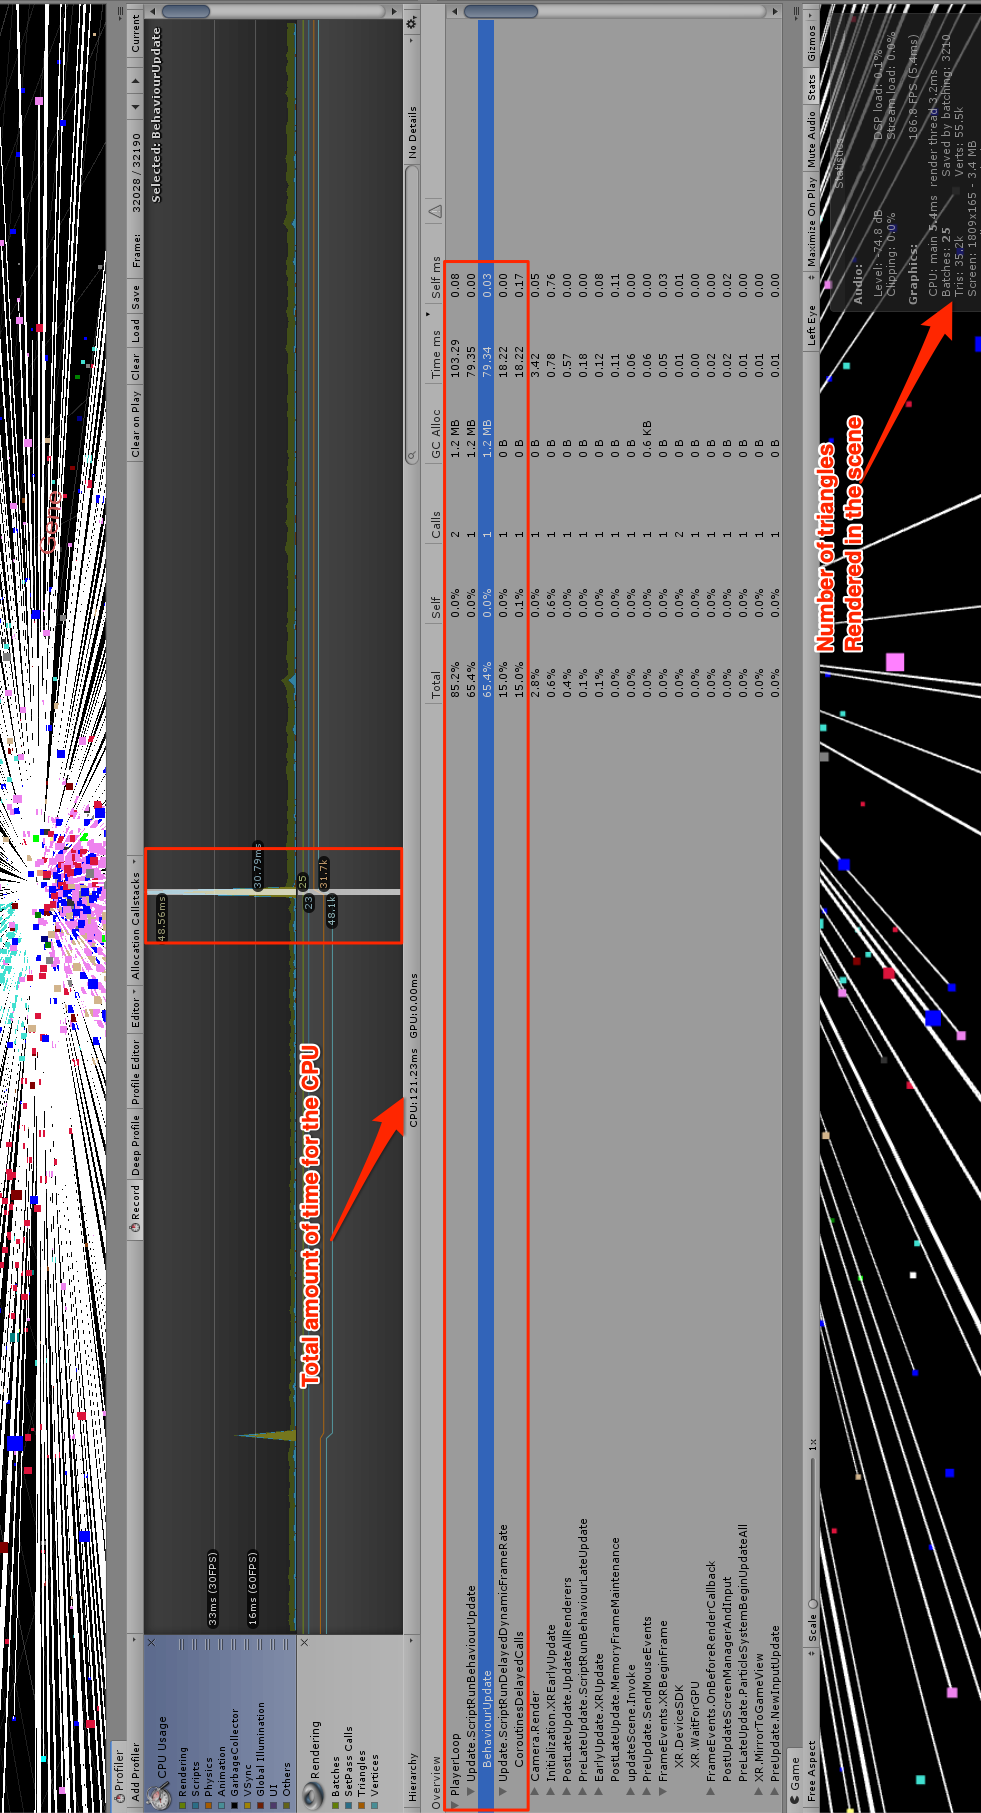
\includegraphics[width=0.9\textwidth]{profiler}
    \caption{Profiling the selection of the node ARGLU1(1607), which has the highest number of edges. We study what is the cause for the high amount of time that this takes to render.}
    \label{fig:profiler}
\end{figure}%

We get also some other metric information from this screenshot (see the region far below and the small black grey square with the Statistics title), like the number of triangles that the scene is rendering. This is the selection of the node with the highest number of edges and there are a total of 35.2k verteces, which is inside of the Oculus' performance guidelines that we mentioned in this chapter.

It's hard to determine from the experiments that we ran, if the number of edges can have an impact in the scalability of the system. We would need to better isolate this part of the code and further evaluate it. However, we expect that the number of edges can have an impact. As we have mentioned before, a better implementation solution could improve the performance of this. Instead of create the edges in the scene every time a node is selected, we can create all the necessary edges in the initialization of the system, and show them when they are needed. So, normally they would be hidden, but we show them when the user selects a node.

% \begin{figure}[h!]
%   \centering
%   \begin{minipage}{.9\textwidth}
%   \begin{tikzpicture}
%     \begin{axis}
%     [ xlabel=Number of edges,
%     ylabel=Time (ms),
%     xmin=0,xmax=430,
%     ymin=0,ymax=100,
%     ]
%     \addplot[only marks, mark=asterisk, color=rred, style={thick}] file{data/scalabilityBiopsy.dat};
%     \end{axis}
%
%     \end{tikzpicture}
%   \end{minipage}
% \caption{Scatter plot showing the relation between the number of edges to render and the time that it takes to render for the biopsy dataset.}
% \label{fig:scalability_edges_biopsy}
% \end{figure}

\section{Do we achieve the recommended FPS (72) for large biological networks when using the standalone Oculus Quest?}
We would like to know if we can use a cheap VR headset like the Oculus Quest to visualize larg biological networks. The hardware for the Oculus Quest is not as good as the machine's, so we expect that the performance in the Oculus Quest will be worse. We also want to know how the performance is improved when using a machine with better hardware.

\begin{figure}[h!]
  \centering
  \begin{minipage}{.8\textwidth}
  \begin{tikzpicture}
    \begin{axis}
    [ xlabel=Frame number,
    ylabel=Time (ms),
    xmin=301,xmax=370,
    ymin=0,ymax=100,
    legend pos=north west,
    ]
    \addplot[color=rred, style={thick}] file{data/headset.dat};
    \addlegendentry{Oculus Quest}
    \addplot[color=bblue, style={thick}] file{data/pc.dat};
    \addlegendentry{PC}
    \draw [ultra thick, dotted]
        (axis cs: 301,13.9) -- (axis cs: 370,13.9)
        node[pos=0.3, above] {72 FPS limit};
    \end{axis}

    \end{tikzpicture}
  \end{minipage}
\caption{Performance of GeneNet VR when visualizing the blood dataset tunning on a machine and on the Oculus Quest. The X axis represents the frame number (like a timeline). The Y axis represents the amount of time in milliseconds that a particular frame took to render.}
\label{fig:pc_vs_oculus}
\end{figure}

We designed an experiment that we could run in both the PC and the Oculus Quest to measure the performance. In this experiment we used combination of the three performance experiments for the interactions and we use them together for this experiment. For a short period of time we translate the network, scale it and select several nodes. The experiment lasts for 70 frames; it starts in frame 300 and ends in frame 370.

In Figure \ref{fig:pc_vs_oculus}, we can see a graph with the results from the experiments. The performance for the Oculus Quest is worse than for the PC, as we had expected; however, most of the frames reach the 72 FPS limit. We can see some peaks in the graph, related to the selection of the nodes. We select a node every 10 frames (7 nodes in total). The nodes are selected in this order (in parenthesis is the number of edges): TGFBR3 (1), EPSTI1(11), SMNDC1(90), HNRNPH3(290), ANGEL2(586) and ACTR6(756).

We can extract from the experiment that we can use GeneNet VR for the network sizes that we used from MIxT and that we achieve the 72 FPS. However, the performance is on the limit of the 72 FPS and when we select nodes with more than 10 edges, the performance can be bad during that frame. It would be necessary evaluate the performance of GeneNet VR using larger networks on the Oculus Quest. Also improve the creationg of the edges as we mentioned before.

\section{How do users perceive the visualization of large biological networks in GeneNet VR?}
One of the questions that we asked ourselves during the evaluation process was about how the users perceive the interactions with the networks. In order to evaluate this we made some interviews to users in order to get feedback about the quality of the application.

Questions related to the locomotion of the VR application:
\begin{itemize}
  \item How do you perceive the application?
  \item How do you perceive the pattern finding?
  \item Is there anything that is missing?
\end{itemize}

Dicussion about the interview:
% The following questionnaire is divided in four sections; a general section about VR headsets, a section about comfortability exploring the network using GeneNet VR, a section about the different actions in GeneNet VR and finally a section about feedback.
%
% To complete the questionnaire, the teste has to indicate the level of agreement or disagreement with each of the  statements, mark yes or no when it is asked and in the feedback section reply the questions with constructive feedback if possible.\\

% TODO Interview questions

% Questionnaire section 1: VR headsets.
% \begin{enumerate}
%   \item Have you ever used a VR headset before?\\
%   Yes / No
%
%   \item Have you ever used a Oculus Quest headset before?\\
%   Yes / No
%
%   \item I feel comfortable using a VR headset.\\
%   Strongly agree / Agree / Neutral / Disagree / Strongly Disagree
%
%   \item I feel comfortable using the Oculus Quest headset.\\
%   Strongly agree / Agree / Neutral / Disagree / Strongly Disagree\\
% \end{enumerate}
%
% Questionnaire section 2: Comfortability exploring a biological network with GeneNet VR.
% \begin{enumerate}
%   \item I feel comfortable moving around the virtual environment using the teleport functionality.\\
%   Strongly agree / Agree / Neutral / Disagree / Strongly Disagree
%
%   \item I feel comfortable rotating to any direction.\\
%   Strongly agree / Agree / Neutral / Disagree / Strongly Disagree
%
%   \item I feel comfortable visualizing the network by moving my head.\\
%   Strongly agree / Agree / Neutral / Disagree / Strongly Disagree
%
%   \item I feel comfortable selecting the nodes to visualize the relationships.\\
%   Strongly agree / Agree / Neutral / Disagree / Strongly Disagree
%
%   \item I feel comfortable moving the network to the position that I want.\\
%   Strongly agree / Agree / Neutral / Disagree / Strongly Disagree
%
%   \item I feel comfortable scaling the network.\\
%   Strongly agree / Agree / Neutral / Disagree / Strongly Disagree
%
%   \item I feel comfortable using the UI menu to filter the data from the network.\\
%   Strongly agree / Agree / Neutral / Disagree / Strongly Disagree\\
% \end{enumerate}
%
% Questionnaire section 3: Performing different actions in GeneNet VR to explore the biological network.
% \begin{enumerate}
%   \item It is intuitive to manipulate the network using the controllers.\\
%   Strongly agree / Agree / Neutral / Disagree / Strongly Disagree
%
%   \item The different actions in the controllers are easy to learn and remember.\\
%   Strongly agree / Agree / Neutral / Disagree / Strongly Disagree
%
%   \item I can move the network to any position that I want.\\
%   Strongly agree / Agree / Neutral / Disagree / Strongly Disagree
%
%   \item I can scale the network to any size that I want.\\
%   Strongly agree / Agree / Neutral / Disagree / Strongly Disagree
%
%   \item I can select any node that I want.\\
%   Strongly agree / Agree / Neutral / Disagree / Strongly Disagree
%
%   \item I can easily visualize the relationships of any node.\\
%   Strongly agree / Agree / Neutral / Disagree / Strongly Disagree
%
%   \item I can easily filter the data by using the UI menu.\\
%   Strongly agree / Agree / Neutral / Disagree / Strongly Disagree\\
% \end{enumerate}
%
% Questionnaire section 4: Feedback.
% \begin{enumerate}
%   \item Did you experience any difficulties exploring the biological network? If so, indicate which ones.\\
%   Yes / No
%
%   \item Is there anything that could be improved for the visualization of biological data in GeneNet VR? If so, write your suggestions.\\
%   Yes / No
%
%   \item Write any feedback and comments that you have about the exploration of biological networks with GeneNet VR.
% \end{enumerate}
